\section{Mesh shader pipeline}

The mesh shader pipeline represents a generalized version of the graphics pipeline where there's no initial fixed part, and mesh generation can be entirely handled by shaders.
\begin{figure}[H]
    \centering
    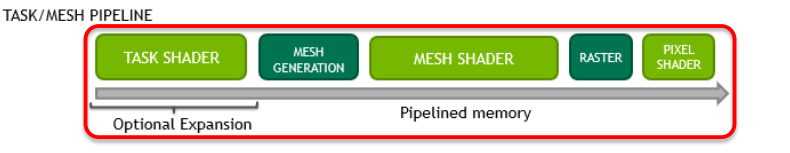
\includegraphics[width=1\linewidth]{images/msp.png}
    \caption{Mesh Shader pipeline}
\end{figure}
Mesh shaders compute indexed triangle lists, providing a set of vertices and groups of three indices for each triangle. 
Vertices are typically computed in normalized screen coordinates to simplify rasterization. 
However, there are limitations on the number of vertices and triangles that a Mesh shader can generate. 
To overcome this limitation, each object is divided into many patches called meshlets.

The optional Task shader plays a crucial role in this pipeline. 
Its purpose is to subdivide a larger mesh into smaller meshlets and control the corresponding mesh shader for generating all the required patches. 
This subdivision helps manage the computational load efficiently.